\begin{filecontents*}{references.bib}
    @article{gilda2020astronomical,
        title={Astronomical Image Quality Prediction based on Environmental and Telescope Operating Conditions},
        author={Gilda, Sankalp and Ting, Yuan-Sen and Withington, Kanoa and Wilson, Matthew and Prunet, Simon and Mahoney, William and Fabbro, Sebastien and Draper, Stark C and Sheinis, Andrew},
        journal={arXiv preprint arXiv:2011.03132},
        year={2020}
    }
    @MISC{JavatpointClassificationAlgImage,
        author = {{Javatpoint}},
        title = {classification algorithm in machine learning},
        url = {https://static.javatpoint.com/tutorial/machine-learning/images/classification-algorithm-in-machine-learning.png}
    }
    @MISC{DavidFumoRegression,
        author = {{David Fumo, Medium}},
        title = {Linear Regression - Intro to Machine Learning},
        url = {https://miro.medium.com/max/1200/1*iuqVEjdtEMY8oIu3cGwC1g.png}
    }
    @MISC{AlFahriz,
        author = {{Al Fahriz, Medium}},
        title = {Mengenal Jenis Pembelajaran Mesin Supervised Learning dan Unsupervised Learning},
        url = {https://medium.com/kelompok1/mengenal-jenis-pembelajaran-mesin-supervised-learning-dan-unsupervised-learning-c588881e8ef5}
    }
    @MISC{TWDSReinforcementLearning,
        author = {{John Cao, Towards Data Science}},
        title = {Reinforcement Learning 101},
        url = {https://towardsdatascience.com/reinforcement-learning-101-e24b50e1d292}
    }
\end{filecontents*}
\documentclass[a4paper,twocolumn]{article}

%%%%%%%%%%%%%%%%%%%%%%%%%%%%%%%%%%%%%%%%%%%%%%%%%%%%%%%%%%%%%%%%%%%%%%
% Document preamble
%%%%%%%%%%%%%%%%%%%%%%%%%%%%%%%%%%%%%%%%%%%%%%%%%%%%%%%%%%%%%%%%%%%%%%

%% Builds upon the graphics  package, providing a key-value interface
%% for optional arguments to the \includegraphics command that go far
%% beyone what the graphics package offers.
%% http://www.ctan.org/tex-archive/help/Catalogue/entries/graphicx.html
%% if you use PostScript figures in your article
%% use the graphics package for simple commands
%% \usepackage{graphics}
%% or use the graphicx package for more complicated commands
%% \usepackage{graphicx}
%% or use the epsfig package if you prefer to use the old commands
%% \usepackage{epsfig}
\usepackage{graphicx} % Enhanced LaTeX Graphics
\graphicspath{{./images/}}
\usepackage[section]{placeins}
\makeatletter
\AtBeginDocument{%
  \expandafter\renewcommand\expandafter\subsection\expandafter{%
    \expandafter\@fb@secFB\subsection
  }%
}
\makeatother

% \usepackage{float}
\usepackage{outlines}
\usepackage{siunitx}
\usepackage{lipsum}
\usepackage[english,bahasai]{babel}%
    \addto{\captionsbahasai}{\renewcommand\refname{Referensi}}
    \addto{\captionsenglish}{\renewcommand\refname{References}}
\usepackage{filecontents}
\usepackage{mathptmx}
% \usepackage{helvet}
% \renewcommand{\familydefault}{\sfdefault}
% \renewcommand{\thesubsection}{\alpha{subsection}}
% acentos e cedilhas
\usepackage[utf8]{inputenc}
%\usepackage[T1]{fontenc}

% Multiple figures
%\usepackage{subfigure} % subcaptions for subfigures
%\usepackage{subfigmat} % matrices of similar subfigures

\usepackage[font=footnotesize, skip = 1pt, labelfont=bf]{caption}
\usepackage[font=footnotesize]{subcaption}

% Declaring new column types
% 'dcolumn' package defines D to be a column specifier with
% three arguments: D{<sep.tex>}{<sep.dvi>}{<decimal places>}
%                  D{<sep.tex>}{<sep.dvi>}{<left digit places>.<right digit places>}
\usepackage{dcolumn}           % decimal-aligned tabular math columns
% d takes a single argument specifying the number of decimal places, e.g., d{2}
% or the number of digits to the left and right of the seperator, e.g., d{3.2}
\newcolumntype{.}   {D{.}{.}{-1}} % column alignedd on the point separator '.'
\newcolumntype{d}[1]{D{.}{.}{#1}} % column centered on the point separator '.'
\newcolumntype{e}   {D{E}{E}{-1}} % column centered on the exponent 'E'
\newcolumntype{E}[1]{D{E}{E}{#1}} % column centered on the exponent 'E'

%% American Mathematical Society (AMS) plain Tex macros
%%
%% The amsmath package is the principal package in the AMS-LaTeX distribution
%% http://www.ctan.org/tex-archive/help/Catalogue/entries/amsmath.html
\usepackage{amsmath}
\DeclareMathSizes{7}{7}{3}{3} 
\usepackage{pifont}
%%
%% The amsfonts package provides extended TeX fonts
%% http://www.ctan.org/tex-archive/help/Catalogue/entries/amsfonts.html
\usepackage{amsfonts}
%% The amssymb package provides various useful mathematical symbols
\usepackage{amssymb}
%%
%% The amsthm package provides extended theorem environments
%% http://www.ctan.org/tex-archive/help/Catalogue/entries/amsthm.html
\usepackage{amsthm}

%% Improves the interface for defining floating objects such as figures and tables.
%% The package also provides the H float modifier option of the obsolete here package.
%% http://www.ctan.org/tex-archive/help/Catalogue/entries/float.html
\usepackage{float}

%% Control sectional headers. 
%% http://www.ctan.org/tex-archive/help/Catalogue/entries/sectsty.html
\usepackage{sectsty}
%%
%% Redefine the font size of the 'section' and 'subsection' headings
\newcommand{\myFontSize}{\fontsize{9}{0}\selectfont}
\sectionfont{\myFontSize}       % 10pt, Bold face (default)
\subsectionfont{\myFontSize} % 10pt, Plain face

%% Select alternative section titles.
%% http://www.ctan.org/tex-archive/help/Catalogue/entries/titlesec.html
\usepackage{titlesec}
\usepackage{booktabs}
%\usepackage{multirow}
%\usepackage{array}
\usepackage[style=english]{csquotes}% Recommended

%\usepackage[style=authoryear, backend=bibtex, doi=false,isbn=false,url=false,eprint=false,dashed=false,maxcitenames=2, maxbibnames=100]{biblatex}
%\addbibresource{library.bib}
% \titleformat*{\section}{\filcenter\bfseries}
\renewcommand{\thesection}{\Roman{section}}
\renewcommand{\thesubsection}{\Alph{subsection}}
\titleformat{\section}[block]{\filcenter\bfseries}{\thesection.}{1em}{}[]
\titleformat{\subsection}[block]{\itshape}{\thesubsection.}{0.5em}{}[]
%%
%% Left indent, before and after spacing
%% (The starred version kills the indentation of the paragraph following the title)
\titlespacing*{\section}{0pt}{10pt}{0pt}
\titlespacing*{\subsection}{0pt}{10pt}{0pt}
\titlespacing*{\subsubsection}{10pt}{0pt}{0pt}



% These are exact settings for a A4 page with top margin of
% 25 mm, bottom margin of 30 mm, left and right margins of 25 mm,
% printable area 242 X 160 mm.

\setlength{\topmargin}{-10.4mm}
\setlength{\headheight}{0.0mm}
\setlength{\headsep}{10.0mm}
\setlength{\textwidth}{160mm}
\setlength{\textheight}{242mm}
\setlength{\oddsidemargin}{0mm}
\setlength{\evensidemargin}{0mm}
\setlength{\marginparwidth}{0mm}
\setlength{\marginparsep}{0mm}

% New command to refer to equations as Eq.(1),Eq.(2),...
\newcommand{\eqnref}[1]{Eq.(\ref{#1})}
%%%%%%%%%%%%%%%%%%%%%%%%%%%%%%%%%%%%%%%%%%%%%%%%%%%%%%%%%%%%%%%%%%%%%%%%%%%%%%%%%%%%%%%%
% Title, authors and addresses

\title{\bfseries Tipe-tipe Algoritma Machine Learning}
\date{13 November 2021}
\author{Ridwan Maulana Tanjung\\ 
        {\small ridwantanjung@student.telkomuniversity.ac.id}\\ \\ 
        \emph{Departemen Teknik Fisika, Universitas Telkom}}

%%%%%%%%%%%%%%%%%%%%%%%%%%%%%%%%%%%%%%%%%%%%%%%%%%%%%%%%%%%%%%%%%%%%%%%%%%%%%%%%%%%%%%%%

\begin{document}
\renewcommand{\abstractname}{Abstrak}


% Begin one column section for title and abstract
%
% http://www.faqs.org/faqs/de-tex-faq/part5/
\twocolumn[
  \begin{@twocolumnfalse}
    \maketitle

    \begin{abstract}
    Machine learning sudah menjadi komponen penting dalam dunia ilmu data yang berkembang.
    Secara luas jenis pembelajaran machine learning terbagi menjadi tiga bagian, yaitu supervised learning, unsupervised learning, dan reinforcement learning.
    Supervised Learning menjadi jenis machine learning paling mendasar, tujuan dari \emph{supervised learning} adalah
    untuk memperoleh kemampuan menggeneralisasi, yang mengacu pada kemampuan bahwa hasil jawaban yang tepat dapat ditebak untuk pertanyaan yang tidak diajarkan.
    \emph{Unsupervised learning} mempertimbangkan situasi dimana tidak ada pengawasan dalam pembelajaran, program mengumpulkan data secara mendiri melalui internet dan mencoba mengekstrak pengetahuan yang bermanfaat tanpa bimbingan dari pengguna.
    Sedangkan \emph{reinforcement learning} mempertimbangkan masalah dan mengarahkan
    pada tujuan saat berinteraksi dengan lingkungan yang tidak pasti.

    \noindent{{\bf keywords:}} Machine Learning, Pembelajaran mesin, Artificial Intelligence
\end{abstract}

  \end{@twocolumnfalse}
]
\section{Pendahuluan}
\label{sec:intro}
\emph{Machine learning} adalah cabang dari kecerdasan buatan dan ilmu komputer yang berfokus
pada penggunaan data dan algoritma untuk meniru cara menusia belajar, dan secara bertahap meningkatkan akurasinya.

Dewasa ini, \emph{machine learning} sudah menjadi komponen penting dalam dunia ilmu data yang berkembang.
Melalui penggunaan metode pemodelan matematika dan statistik, algoritma dilatihan untuk mengklasifikasikan dan memprediksikan sesuatu
berdasarkan \emph{set} data yang ada. Penggunaan \emph{machine learning} tidak hanya terbatas pada bidang ilmu komputer, tetapi lebih luas lagi seperti pada
ilmu fisika, astronomi, biologi, ekonomi, dan bisnis. Pada ilmu astronomi contohnya, \emph{machine learning} digunakan untuk meningkatkan kualitas gambar saat pengambilan gambar objek asing di luar angkasa \cite{gilda2020astronomical}.
\section{Jenis Pembelajaran}
Ada beberapa jenis pembelajaran yang dimiliki oleh \emph{machine learing}, itu tergantung pada jenis data yang tersedia. Namun secara luas jenis pembelajaran
\emph{machine learning} terbagi menjadi tiga bagian, yaitu \emph{supervised learning}, \emph{unsupervised learning}, dan \emph{reinforcement learning}.
\subsection{Supervised Learning}
Supervised learning menjadi jenis \emph{machine learning} paling mendasar. Dalam konteks ini tujuan dari \emph{supervised learning} adalah
untuk memperoleh kemampuan menggeneralisasi, yang mengacu pada kemampuan bahwa hasil jawaban yang tepat dapat ditebak untuk pertanyaan yang tidak diajarkan.
Dengan demikian, pengguna tidak harus mengajarkan semuanya ke program, tetapi program dapat secara otomatis mengatasi situasi yang tidak diketahui dengan hanya mempelajari
sebagian kecil pengetahuan saja.

Algoritma yang tergolong \emph{supervised learning} biasanya digunakan untuk menyelesaikan berbagai persoalan yang berkaitan dengan:
\begin{itemize}
    \item  \emph{Classification} (Klasifikasi)

          \emph{Classification} dapat didefinisikan sebagai proses memprediksi kelas atau kategori dari nilai yang diamati
          atau titik data yang diberikan. Ada dua jenis tipe \emph{classification} yaitu \emph{Binary Classifier} dan \emph{Multi-class Classifier}.

          Secara matematis, \emph{classification} adalah tugas pemetaan fungsi $(f)$ dari variabel \emph{input} $(x)$ ke variabel \emph{output} $(y)$
          \begin{figure}[h]
              \centering
              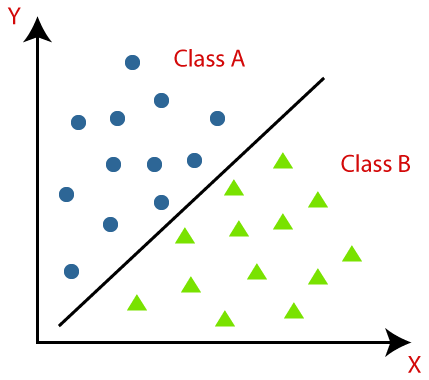
\includegraphics[scale=0.25]{classification-algorithm}
              \caption{Classification algorithm \cite{JavatpointClassificationAlgImage}}
          \end{figure}
    \item  \emph{Regression} (Regresi)

          \emph{Regression} dapat didefinisikan sebagai suatu metode analisis statistik yang digunakan agar dapat melihat pengaruh antara dua variabel atau lebih.
          Hubungan variabel yang dimaksud bersifat fungsional yang diwujudkan dalam bentuk model matematis.
          Pada analisis regresi, variabel dibagi menjadi dua jenis yaitu variabel respons atau biasa disebut variabel bergantung dan variabel bebas atau dikenal dengan istilah variabel independen.
          Ada beberapa jenis analisis regresi yaitu regresi sederhana meliputi regresi linier sederhana dan non-linier sederhana dan regresi berganda meliputi linier berganda atau non-linier berganda.
          \begin{figure}[h]
              \centering
              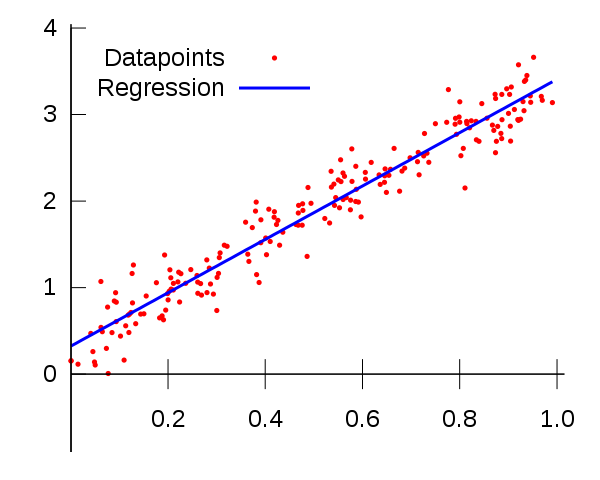
\includegraphics[scale=0.25]{regression-algorithm}
              \caption{Regression algorithm \cite{DavidFumoRegression}}
          \end{figure}
\end{itemize}
\subsection{Unsupervised Learning}
\emph{Unsupervised learning} mempertimbangkan situasi dimana tidak ada pengawasan dalam pembelajaran. Dalam konteks ini, program mengumpulkan data secara mendiri melalui internet dan mencoba mengekstrak pengetahuan yang bermanfaat tanpa bimbingan dari pengguna.
Konsep yang metode ini gunakan jauh berbeda dengan metode \emph{supervised learning} dimana pada metode ini hasil yang diharapkan tidak dapat diketahui oleh siapapun.
Dengan kata lain, hasil yang akan ditampilkan hanya bergantung kepada nilai bobot yang disusun pada awal pembangunan sistem dan tentu masih dalam ruang lingkup tertentu.

Contoh Studi Kasus pemecahan masalah dengan metode \emph{unsupervised learning} adalah misal suatu pusat perbelanjaan ingin melakukan bongkar muat terhadap satu truk berisi sepatu campur.
Agar dapat dijual sepatu-sepatu tersebut perlu dikelompokkan brand dan ukurannya.
Dalam hal ini, pihak pusat perbelanjaan tidak perlu memasukkan datanya terlebih dahulu karena data yang ada dilapangan saat itulah yang langsung diproses untuk mengelompokkan sepatu-sepatu tersebut sesuai brand dan ukurannya\cite{AlFahriz}.
\begin{figure}[h]
    \centering
    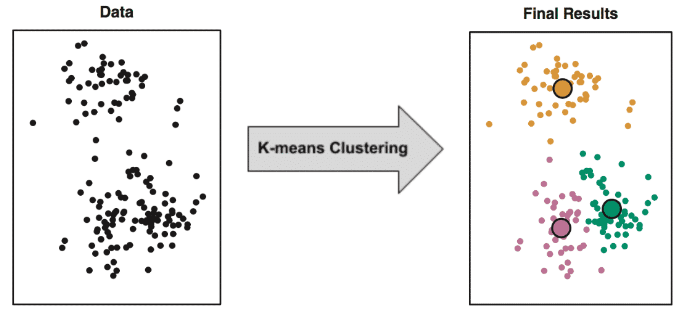
\includegraphics[scale=0.25]{unsupervised-learning}
    \caption{Unsupervised Learning \cite{AlFahriz}}
\end{figure}

\subsection{Reinforcement Learning}
\emph{Reinforcement learning} bertujuan untuk memperoleh kemampuan generalisasi dalam cara yang sama seperti \emph{supervised learning}.
Bedanya, \emph{supervisor} tidak memberikan solusi atau jawaban secara langsung. Sebaliknya, \emph{supervisor} hanya mengevaluasi perilaku program (agen) dan memberikan \emph{feedback}.
Dibandingkan dengan \emph{supervised learning}, \emph{reinforcement learning} berbeda dalam hal tujuan, dalam kasus \emph{reinforcement learning} tujuannya adalah untuk menemukan model tindakan yang sesuai yang akan memaksimalkan total \emph{cumulative reward} agen.
Dengan kata lain
\emph{reinforcement learning} adalah mempertimbangkan masalah dan mengarahkan
pada tujuan saat berinteraksi dengan lingkungan yang tidak pasti. Agen
menerima state(representasi dari enviroment) dan memilih action. Selanjutnya
agent akan menerima nilai reward dari action yang dipilih. Agen akan berusaha
memaksimalkan reward yang diterima dari waktu ke waktu.
\begin{figure}[h]
    \centering
    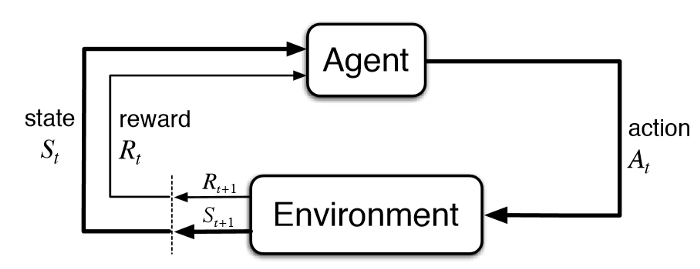
\includegraphics[scale=0.25]{reinforcement-learning}
    \caption{Reinforcement Learning \cite{TWDSReinforcementLearning}}
\end{figure}
% \input{03_theory}

% REFERENCES

% Produces the bibliography section when processed by BibTeX
%
% Bibliography style
% > entries ordered alphabetically
%\bibliographystyle{plain}
% > unsorted with entries appearing in the order in which the citations appear.
\bibliographystyle{unsrt}
% > entries ordered alphabetically, with first names and names of journals and months abbreviated
% \bibliographystyle{abbrv}
% > entries ordered alphabetically, with reference markers based on authors' initials and publication year
%\bibliographystyle{alpha}
% \bibliographystyle{IEEEtranN}

% External bibliography database file in the BibTeX format (ExtendedAbstract_ref_db.bib)
\bibliography{references}

\end{document}